  %%%%%%%%%%%%%%%%%%%%%%%%%%%%%%%%%%%%%%% -*- coding: utf-8; mode: latex -*- %%
  %
%%%%%                        CHAPTER
 %%%
  %

% $Id: 1120-facere-possimus.tex,v 1.1 2007/11/23 09:52:40 david Exp $
% $Log: 1120-facere-possimus.tex,v $
% Revision 1.1  2007/11/23 09:52:40  david
% *** empty log message ***
%
%

  %%%%%%%%%%%%%%%%%%%%%%%%%%%%%%%%%%%%%%%%%%%%%%%%%%%%%%%%%%%%%%%%%%%%%%%%%%%%%
  %
%%%%%                            HEAD MATTER
 %%%
  %

\chapter{Background and Related Work}
%\addcontentsline{lof}{chapter}{\thechapter\quad Facere Possimus}
%\addcontentsline{lot}{chapter}{\thechapter\quad Facere Possimus}
\label{ch:Background}

%\begin{quotation}
%  {\small\it Neque porro quisquam est qui dolorem ipsum quia dolor sit amet, consectetur, adipisci velit...}
%
%{\small\it -- Cerico}
%\end{quotation}




  %%%%%%%%%%%%%%%%%%%%%%%%%%%%%%%%%%%%%%%%%%%%%%%%%%%%%%%%%%%%%%%%%%%%%%%%%%%%%
  %
%%%%%                        FIRST SECTION
 %%%
  %

\section{Distributed File Systems}

Distributed File systems is the fundamental in big data era. They provide a high available storage service with fault tolerance for data corruption, which enable petabytes of data to be persisted across multiple low cost commodity machines reliably.

\subsection{The Google File System}

\textit{The Google File System} (GFS) is a scalable distributed file system developed and widely used in \textit{Google Incorporation} for large distributed data-intensive applications. With fault tolerance, it runs on clusters of inexpensive commodity hardware, which provides a storage layer for a large number of applications with high aggregate performance~\cite{ghemawat2003google}. There are some design assumptions for the implementation of GFS:

\begin{itemize}
	\item The system runs on top on inexpensive commodity hardware so component may often fails.
	\item Files stored on the system are fairly huge than the transitional standards, which means that Gigabyte files are common.
	\item There are three kinds of workloads in the system: large streaming reads, small random reads and large sequential writes which append data to files.
	\item Efficiently well-defined semantics for concurrent appends to the same file is needed.
	\item Data processing in bulk with high sustained bandwidth is more important than individual read or write with low latency.
\end{itemize}

\noindent The architecture of a GFS cluster consists of a single \textit{master}, multiple \textit{chunkservers}, and is accessed by multiple \textit{clients} as shown in Figure~\ref{fig:gfs}.

\begin{figure}[ht]
	\centering
	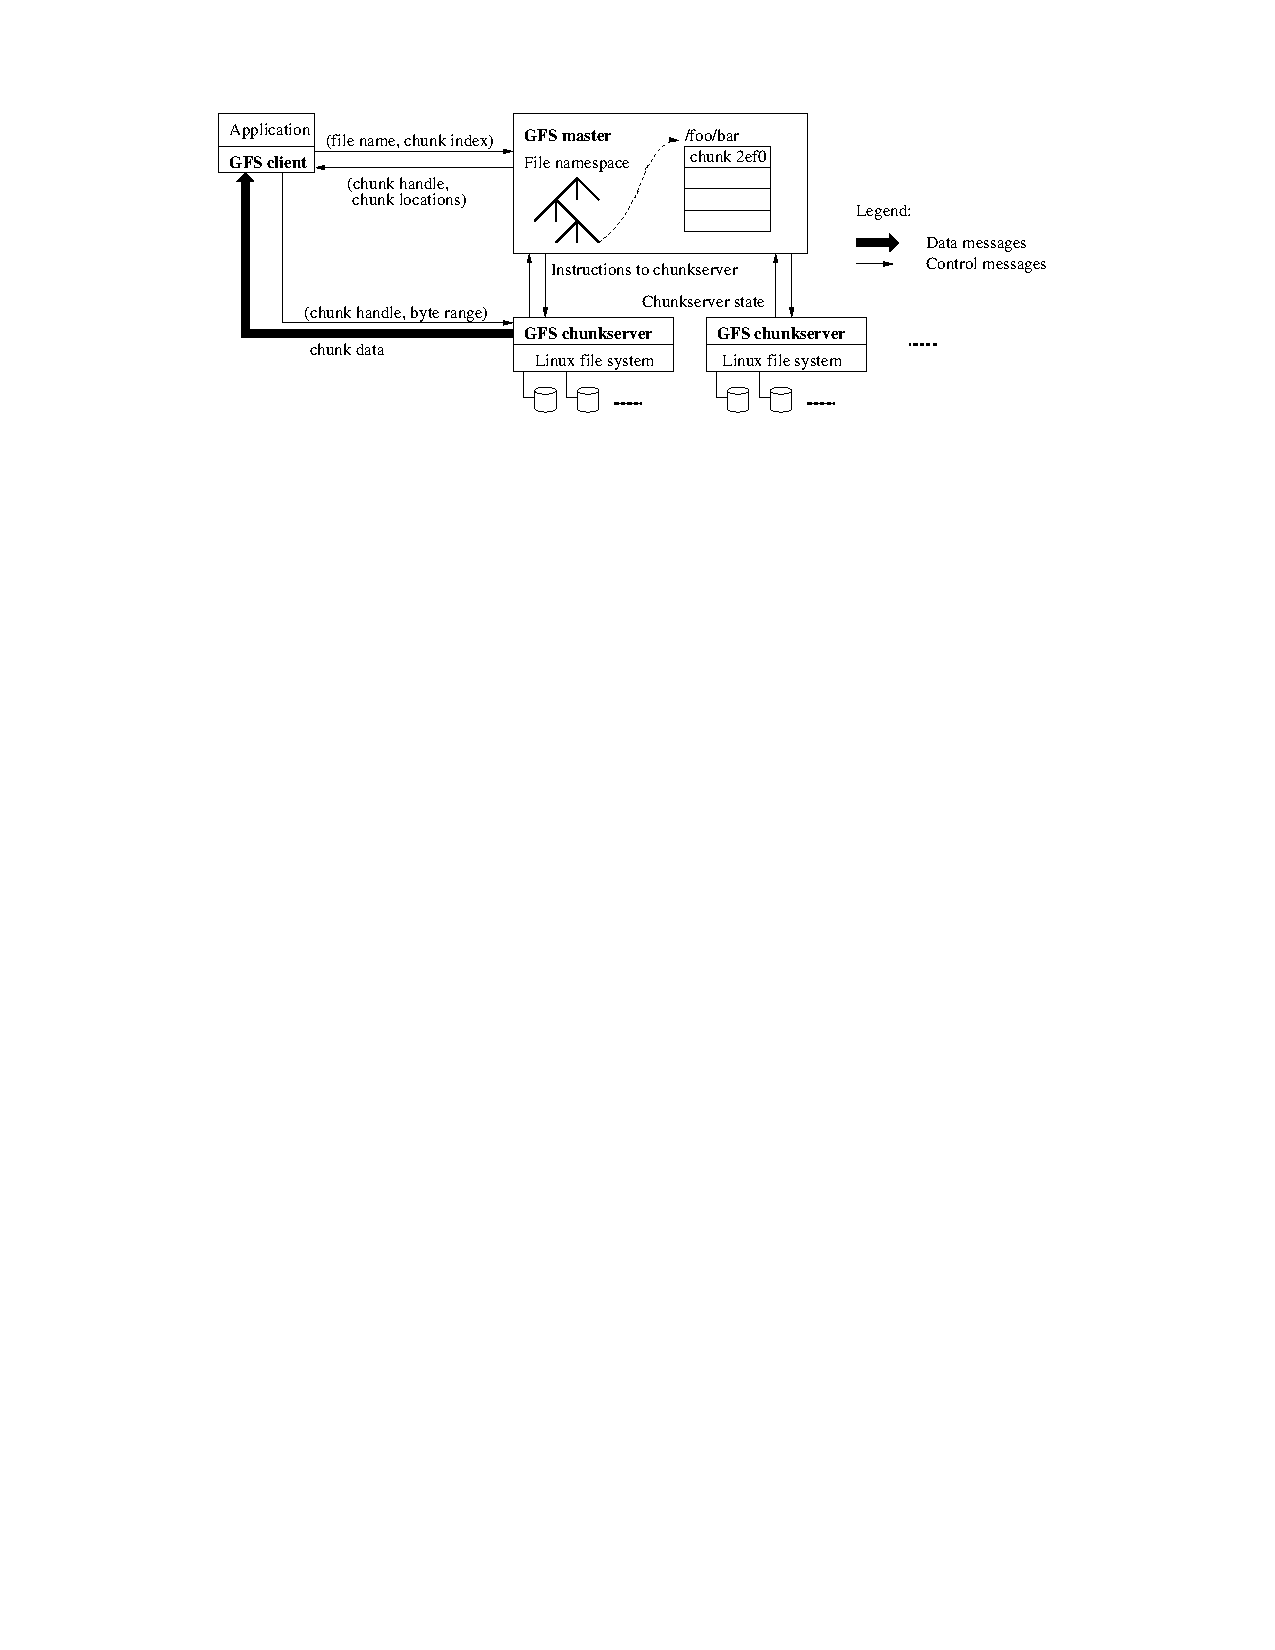
\includegraphics[width=\linewidth]{figs/GFSArchitecture.pdf}
	\caption{The Architecture of GFS \protect \cite{ghemawat2003google}}
	\label{fig:gfs}
\end{figure}

\noindent Files are divided into fixed size \textit{chunks} stored in \textit{chunkservers}. For fault tolerance, each chunk is replicated across multiple chunkservers and the default replication factor is three.

\noindent The \textit{master} is a metadata server maintaining namespace, access control information, the file-chunk mappings and chunks' current locations. Besides, it is also responsible for system-wide activities including garbage collection, chunk lease management, chunk migration between chunkservers.

\noindent Although this single master server architecture simplifies the design of GFS, especially on complexed tasks like chunk placement and replication decisions using global knowledge, yet the master's involvement in reads and writes needs to be minimized otherwise it will become a bottleneck in the system.

\subsection{The Hadoop Distributed File System}

The \textit{Hadoop Distributed File System} (HDFS) is inspired by the Google File System. Initially, HDFS is built for Hadoop Map-Reduce computational framework. With the development of Hadoop ecosystem including HBase~\cite{apachehbase}, Pig~\cite{apachepig}, Mahout~\cite{apachemahout}, Spark~\cite{apachespark}, etc, HDFS becomes the storage layer for other big data applications. Enabling petabytes of data to be persisted on clusters of commodity hardware at relatively low cost, HDFS aims to stream these large data sets at high bandwidth to user applications. Therefore, like GFS, HDFS is optimized for delivering a high throughput of data at the expense of latency~\cite{white2012hadoop}.

\noindent Similar to GFS, HDFS stores metadata and file data separately. The architecture of a HDFS cluster consists of a single \textit{NameNode}, multiple \textit{DataNodes}, and is accessed by multiple \textit{clients} as shown in Figure~\ref{fig:hdfsv1}.

\begin{figure}[ht]
	\centering
	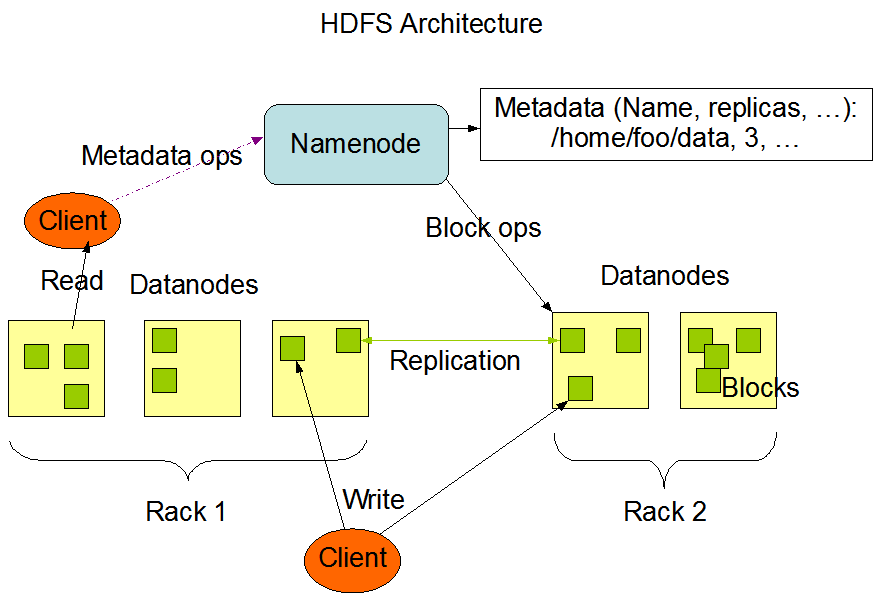
\includegraphics[scale=0.4]{figs/hdfsarchitecturev1.png}
	\caption{The Architecture of HDFS \protect \cite{borthakur2008hdfs}}
	\label{fig:hdfsv1}
\end{figure}

\noindent Files in HDFS are split into smaller blocks stored in \textit{DataNodes}. For fault tolerance, each block is replicated across multiple \textit{DataNodes}.

\noindent The \textit{NameNode} is a single dedicated metadata server maintaining the namespace, access control information, and file blocks mappings to DataNodes. The entire namespace is kept in-memory, called the \textit{image}, of the \textit{NameNode}. Its related persistent record, called the \textit{checkpoint} is stored in the local physical file system. The modification, \textit{editlogs}, of the \textit{image}, called the \textit{journal}, is also persisted in the local physical file system. Copies of the \textit{checkpoints} and the \textit{journals} can made at other servers for durability. Therefore, the \textit{NameNode} restores the namespace by loading the checkpoint and replaying the journal during its restart.
  %%%%%%%%%%%%%%%%%%%%%%%%%%%%%%%%%%%%%%%%%%%%%%%%%%%%%%%%%%%%%%%%%%%%%%%%%%%%%
  %
%%%%%                      SECOND SECTION
 %%%
  %

\section{Concurrency Control in Transactional Systems}

BBB

  %%%%%%%%%%%%%%%%%%%%%%%%%%%%%%%%%%%%%%%%%%%%%%%%%%%%%%%%%%%%%%%%%%%%%%%%%%%%%
  %
%%%%%                         ANOTHER SECTION
 %%%
  %
\section{Isolation Level in Transactional Systems}

CCC

  %%%%%%%%%%%%%%%%%%%%%%%%%%%%%%%%%%%%%%%%%%%%%%%%%%%%%%%%%%%%%%%%%%%%%%%%%%%%%
  %
%%%%%                          LAST SECTION
 %%%
  %

\section{MySQL Cluster}

DDD

  %
 %%%
%%%%%                            THE END
  %
  %%%%%%%%%%%%%%%%%%%%%%%%%%%%%%%%%%%%%%%%%%%%%%%%%%%%%%%%%%%%%%%%%%%%%%%%%%%%%

%%% Local Variables: 
%%% mode: latex
%%% TeX-master: "tese"
%%% End: 
